
\chapter{Flip-book animations}

This appendix demonstrates certain principles through the use of ``flip-book'' animation.  Each page of these appendix sections forms one frame of the ``animation,'' viewed by rapidly flipping pages (if the book is printed), or rapidly clicking the ``next page'' button (if the book is viewed on a computer).  While crude, this animation technique enjoys the benefits of low technology (it even works in paper form!) and convenient pausing at critical frames.

\vskip 10pt

Enjoy!








\filbreak
\section{Polyphase light bulbs animated}

The key to understanding how three-phase electric motors work is to have an accurate mental picture of the \textit{rotating magnetic field} created by the stator windings of a polyphase motor.  One of the best ways to visualize this phenomenon is to observe a string of ``chaser'' lights blinking in a polyphase sequence.  Just in case you don't happen to have a string of polyphase lights at your viewing convenience, I have provided a simulation here to demonstrate how the illusion of motion is created by the sequential energization of light bulbs.  \index{Rotating magnetic field}   \index{Induction motor}  \index{AC induction motor} 

Note how the lights appear to ``move'' from left to right as the energization sequences moves from A to C.  After a few cycles of \texttt{ABC}, two of the wires are crossed to reverse phase sequence.  This has the result of reversing the apparent direction of motion!  It matters not which two phases are reversed.  In this animation, I reverse phases A and B, but I could have just as well swapped phases B and C, or phases A and C, and created the exact same effect.

\label{animation_blinking_lights}

\vfil \eject
$$\includegraphics[width=6in]{lights_01.eps}$$

\vfil \eject
$$\includegraphics[width=6in]{lights_02.eps}$$

\vfil \eject
$$\includegraphics[width=6in]{lights_03.eps}$$

\vfil \eject
$$\includegraphics[width=6in]{lights_01.eps}$$

\vfil \eject
$$\includegraphics[width=6in]{lights_02.eps}$$

\vfil \eject
$$\includegraphics[width=6in]{lights_03.eps}$$

\vfil \eject
$$\includegraphics[width=6in]{lights_01.eps}$$

\vfil \eject
$$\includegraphics[width=6in]{lights_02.eps}$$

\vfil \eject
$$\includegraphics[width=6in]{lights_03.eps}$$

\vfil \eject
$$\includegraphics[width=6in]{lights_01.eps}$$

\vfil \eject
$$\includegraphics[width=6in]{lights_02.eps}$$

\vfil \eject
$$\includegraphics[width=6in]{lights_03.eps}$$

\vfil \eject
$$\includegraphics[width=6in]{lights_04.eps}$$

\vfil \eject
$$\includegraphics[width=6in]{lights_05.eps}$$

\vfil \eject
$$\includegraphics[width=6in]{lights_06.eps}$$

\vfil \eject
$$\includegraphics[width=6in]{lights_07.eps}$$

\vfil \eject
$$\includegraphics[width=6in]{lights_08.eps}$$

\vfil \eject
$$\includegraphics[width=6in]{lights_06.eps}$$

\vfil \eject
$$\includegraphics[width=6in]{lights_07.eps}$$

\vfil \eject
$$\includegraphics[width=6in]{lights_08.eps}$$

\vfil \eject
$$\includegraphics[width=6in]{lights_06.eps}$$

\vfil \eject
$$\includegraphics[width=6in]{lights_07.eps}$$

\vfil \eject
$$\includegraphics[width=6in]{lights_08.eps}$$

\vfil \eject
$$\includegraphics[width=6in]{lights_06.eps}$$

\vfil \eject
$$\includegraphics[width=6in]{lights_07.eps}$$

\vfil \eject
$$\includegraphics[width=6in]{lights_08.eps}$$














\vfil \eject
\section{Polyphase induction motor animated}

The following animation shows how the ``rotating'' magnetic field of a three-phase AC induction motor is produced by the interaction of three stator winding sets energized with different phases (A, B, and C) of a three-phase AC power source.  A red arrow shows the direction of the \textit{resultant} magnetic field created by the interaction of the three winding sets.

\label{animation_3phase_motor}

\vfil \eject
$$\includegraphics[width=6in]{03232x01.eps}$$

\vfil \eject
$$\includegraphics[width=6in]{03232x02.eps}$$

\vfil \eject
$$\includegraphics[width=6in]{03232x03.eps}$$

\vfil \eject
$$\includegraphics[width=6in]{03232x04.eps}$$

\vfil \eject
$$\includegraphics[width=6in]{03232x05.eps}$$

\vfil \eject
$$\includegraphics[width=6in]{03232x06.eps}$$

\vfil \eject
$$\includegraphics[width=6in]{03232x07.eps}$$

\vfil \eject
$$\includegraphics[width=6in]{03232x08.eps}$$

\vfil \eject
$$\includegraphics[width=6in]{03232x09.eps}$$

\vfil \eject
$$\includegraphics[width=6in]{03232x10.eps}$$

\vfil \eject
$$\includegraphics[width=6in]{03232x11.eps}$$

\vfil \eject
$$\includegraphics[width=6in]{03232x12.eps}$$

\vfil \eject
$$\includegraphics[width=6in]{03232x01.eps}$$

\vfil \eject
$$\includegraphics[width=6in]{03232x02.eps}$$

\vfil \eject
$$\includegraphics[width=6in]{03232x03.eps}$$

\vfil \eject
$$\includegraphics[width=6in]{03232x04.eps}$$

\vfil \eject
$$\includegraphics[width=6in]{03232x05.eps}$$

\vfil \eject
$$\includegraphics[width=6in]{03232x06.eps}$$

\vfil \eject
$$\includegraphics[width=6in]{03232x07.eps}$$

\vfil \eject
$$\includegraphics[width=6in]{03232x08.eps}$$

\vfil \eject
$$\includegraphics[width=6in]{03232x09.eps}$$

\vfil \eject
$$\includegraphics[width=6in]{03232x10.eps}$$

\vfil \eject
$$\includegraphics[width=6in]{03232x11.eps}$$

\vfil \eject
$$\includegraphics[width=6in]{03232x12.eps}$$















\vfil \eject
\section{Rotating phasor animated}

The following animation shows a rotating phasor in three-dimensional form.  The phasor rotates in a complex plane (with real and imaginary axes), but travels linearly along the time axis.  In doing so it traces a path that looks like a circle when viewed along the centerline (time axis) but looks like a sinusoidal wave when viewed from above or along the side.

\label{animation_rotating_phasor}

\vskip 10pt

Euler's Relation describes the phasor's position in the complex plane:

$$e^{j \omega t} = \cos \omega t + j \sin \omega t$$

\noindent
Where,

$e$ = Euler's number (approximately equal to 2.718281828)

$\omega$ = Angular velocity, in radians per second

$t$ = Time, in seconds

$\cos \omega t$ = Horizontal projection of phasor (along a real number line) at time $t$

$j \sin \omega t$ = Vertical projection of phasor (along an imaginary number line) at time $t$

\vskip 40pt

If you imagine the phasor's length either growing or decaying exponentially over time, the result will be a spiral that either widens like a horn or shrinks like a funnel.  This would be a visualization of a \textit{complex} exponential, where the $s$ variable defines both the rate of growth/decay (the envelope of the spiral) and the angular velocity (the pitch of the spiral):

$$e^{st} = e^{(\sigma + j\omega)t} = e^{\sigma t} e^{j \omega t}$$

\noindent
Where,

$s$ = Complex growth/decay rate and frequency (sec$^{-1}$)

$\sigma$ = $1 \over \tau$ = Real growth/decay rate (time constants per second, or sec$^{-1}$)

$j \omega$ = Imaginary frequency (radians per second, or sec$^{-1}$)

$t$ = Time (seconds)

\vskip 10pt

The example of a unit-length rotating phasor is nothing more than a special case of the complex exponential, where $\sigma = 0$ (i.e. there is no growth or decay over time):

$$e^{st} = e^{(0 + j\omega)t} = e^{0} e^{j \omega t} = e^{j \omega t}$$



\vfil \eject
$$\includegraphics[width=6in]{phasor_01.eps}$$

\vfil \eject
$$\includegraphics[width=6in]{phasor_02.eps}$$

\vfil \eject
$$\includegraphics[width=6in]{phasor_03.eps}$$

\vfil \eject
$$\includegraphics[width=6in]{phasor_04.eps}$$

\vfil \eject
$$\includegraphics[width=6in]{phasor_05.eps}$$

\vfil \eject
$$\includegraphics[width=6in]{phasor_06.eps}$$

\vfil \eject
$$\includegraphics[width=6in]{phasor_07.eps}$$

\vfil \eject
$$\includegraphics[width=6in]{phasor_08.eps}$$

\vfil \eject
$$\includegraphics[width=6in]{phasor_09.eps}$$

\vfil \eject
$$\includegraphics[width=6in]{phasor_10.eps}$$

\vfil \eject
$$\includegraphics[width=6in]{phasor_11.eps}$$

\vfil \eject
$$\includegraphics[width=6in]{phasor_12.eps}$$

\vfil \eject
$$\includegraphics[width=6in]{phasor_13.eps}$$

\vfil \eject
$$\includegraphics[width=6in]{phasor_14.eps}$$

\vfil \eject
$$\includegraphics[width=6in]{phasor_15.eps}$$

\vfil \eject
$$\includegraphics[width=6in]{phasor_16.eps}$$

\vfil \eject
$$\includegraphics[width=6in]{phasor_17.eps}$$

\vfil \eject
$$\includegraphics[width=6in]{phasor_18.eps}$$

\vfil \eject
$$\includegraphics[width=6in]{phasor_19.eps}$$

\vfil \eject
$$\includegraphics[width=6in]{phasor_20.eps}$$

\vfil \eject
$$\includegraphics[width=6in]{phasor_21.eps}$$

\vfil \eject
$$\includegraphics[width=6in]{phasor_22.eps}$$

\vfil \eject
$$\includegraphics[width=6in]{phasor_23.eps}$$

\vfil \eject
$$\includegraphics[width=6in]{phasor_24.eps}$$

\vfil \eject
$$\includegraphics[width=6in]{phasor_25.eps}$$

\vfil \eject
$$\includegraphics[width=6in]{phasor_26.eps}$$

\vfil \eject
$$\includegraphics[width=6in]{phasor_27.eps}$$

\vfil \eject
$$\includegraphics[width=6in]{phasor_28.eps}$$

\vfil \eject
$$\includegraphics[width=6in]{phasor_29.eps}$$

\vfil \eject
$$\includegraphics[width=6in]{phasor_30.eps}$$

\vfil \eject
$$\includegraphics[width=6in]{phasor_31.eps}$$

\vfil \eject
$$\includegraphics[width=6in]{phasor_32.eps}$$

\vfil \eject
$$\includegraphics[width=6in]{phasor_33.eps}$$

\vfil \eject
$$\includegraphics[width=6in]{phasor_34.eps}$$

\vfil \eject
$$\includegraphics[width=6in]{phasor_35.eps}$$

\vfil \eject
$$\includegraphics[width=6in]{phasor_36.eps}$$

\vfil \eject
$$\includegraphics[width=6in]{phasor_37.eps}$$

\vfil \eject
$$\includegraphics[width=6in]{phasor_38.eps}$$

\vfil \eject
$$\includegraphics[width=6in]{phasor_39.eps}$$

\vfil \eject
$$\includegraphics[width=6in]{phasor_40.eps}$$
















\vfil \eject
\section{Differentiation and integration animated}

The following animation shows the calculus concepts of differentiation and integration (with respect to time) applied to the filling and draining of a water tank.

\label{animation_calculus_tankfilling}

The animation shows two graphs relating to the water storage tank: one showing the volume of stored water in the tank ($V$) and the other showing volumetric flow rate in and out of the tank ($Q$).  We know from calculus that volumetric flow rate is the \textit{time-derivative} of volume:

$$Q = {dV \over dt}$$

We also know that change in volume is the \textit{time-integral} of volumetric flow rate:

$$\Delta V = \int_{t_0}^{t_1} Q \> dt$$

Thus, the example of a water storage tank filling and draining serves to neatly illustrate both concepts in relation to each other.



\vfil \eject
$$\includegraphics[width=6in]{04090x01_00.eps}$$

\vfil \eject
$$\includegraphics[width=6in]{04090x01_05.eps}$$

\vfil \eject
$$\includegraphics[width=6in]{04090x02_00.eps}$$

\vfil \eject
$$\includegraphics[width=6in]{04090x02_05.eps}$$

\vfil \eject
$$\includegraphics[width=6in]{04090x03_00.eps}$$

\vfil \eject
$$\includegraphics[width=6in]{04090x03_05.eps}$$

\vfil \eject
$$\includegraphics[width=6in]{04090x04_00.eps}$$

\vfil \eject
$$\includegraphics[width=6in]{04090x04_05.eps}$$

\vfil \eject
$$\includegraphics[width=6in]{04090x05_00.eps}$$

\vfil \eject
$$\includegraphics[width=6in]{04090x05_05.eps}$$

\vfil \eject
$$\includegraphics[width=6in]{04090x06_00.eps}$$

\vfil \eject
$$\includegraphics[width=6in]{04090x06_05.eps}$$

\vfil \eject
$$\includegraphics[width=6in]{04090x07_00.eps}$$

\vfil \eject
$$\includegraphics[width=6in]{04090x07_05.eps}$$

\vfil \eject
$$\includegraphics[width=6in]{04090x08_00.eps}$$

\vfil \eject
$$\includegraphics[width=6in]{04090x08_05.eps}$$

\vfil \eject
$$\includegraphics[width=6in]{04090x09_00.eps}$$

\vfil \eject
$$\includegraphics[width=6in]{04090x09_05.eps}$$

\vfil \eject
$$\includegraphics[width=6in]{04090x10_00.eps}$$

\vfil \eject
$$\includegraphics[width=6in]{04090x10_05.eps}$$

\vfil \eject
$$\includegraphics[width=6in]{04090x11_00.eps}$$

\vfil \eject
$$\includegraphics[width=6in]{04090x11_05.eps}$$

\vfil \eject
$$\includegraphics[width=6in]{04090x12_00.eps}$$

\vfil \eject
$$\includegraphics[width=6in]{04090x12_05.eps}$$

\vfil \eject
$$\includegraphics[width=6in]{04090x13_00.eps}$$

\vfil \eject
$$\includegraphics[width=6in]{04090x13_05.eps}$$

\vfil \eject
$$\includegraphics[width=6in]{04090x14_00.eps}$$

\vfil \eject
$$\includegraphics[width=6in]{04090x14_05.eps}$$

\vfil \eject
$$\includegraphics[width=6in]{04090x15_00.eps}$$

\vfil \eject
$$\includegraphics[width=6in]{04090x15_05.eps}$$

\vfil \eject
$$\includegraphics[width=6in]{04090x16_00.eps}$$

\vfil \eject
$$\includegraphics[width=6in]{04090x16_05.eps}$$

\vfil \eject
$$\includegraphics[width=6in]{04090x17_00.eps}$$

\vfil \eject
$$\includegraphics[width=6in]{04090x17_05.eps}$$

\vfil \eject
$$\includegraphics[width=6in]{04090x18_00.eps}$$

\vfil \eject
$$\includegraphics[width=6in]{04090x18_05.eps}$$

\vfil \eject
$$\includegraphics[width=6in]{04090x19_00.eps}$$

\vfil \eject
$$\includegraphics[width=6in]{04090x19_05.eps}$$

\vfil \eject
$$\includegraphics[width=6in]{04090x20_00.eps}$$

\vfil \eject
$$\includegraphics[width=6in]{04090x20_05.eps}$$

\vfil \eject
$$\includegraphics[width=6in]{04090x21_00.eps}$$

\vfil \eject
$$\includegraphics[width=6in]{04090x21_05.eps}$$

\vfil \eject
$$\includegraphics[width=6in]{04090x22_00.eps}$$

\vfil \eject
$$\includegraphics[width=6in]{04090x22_05.eps}$$

\vfil \eject
$$\includegraphics[width=6in]{04090x23_00.eps}$$ % Introduce explanatory text and pause

\vfil \eject
$$\includegraphics[width=6in]{04090x23_05.eps}$$

% Begin showing tangent line slope and derivative height:

\vfil \eject
$$\includegraphics[width=6in]{04090x24_00.eps}$$ 

\vfil \eject
$$\includegraphics[width=6in]{04090x24_05.eps}$$ 

\vfil \eject
$$\includegraphics[width=6in]{04090x25_00.eps}$$ 

\vfil \eject
$$\includegraphics[width=6in]{04090x25_05.eps}$$ 

\vfil \eject
$$\includegraphics[width=6in]{04090x26_00.eps}$$ 

\vfil \eject
$$\includegraphics[width=6in]{04090x26_05.eps}$$ 

\vfil \eject
$$\includegraphics[width=6in]{04090x27_00.eps}$$ 

\vfil \eject
$$\includegraphics[width=6in]{04090x27_05.eps}$$ 

\vfil \eject
$$\includegraphics[width=6in]{04090x28_00.eps}$$ 

\vfil \eject
$$\includegraphics[width=6in]{04090x28_05.eps}$$ 

\vfil \eject
$$\includegraphics[width=6in]{04090x29_00.eps}$$ 

\vfil \eject
$$\includegraphics[width=6in]{04090x29_05.eps}$$ 

\vfil \eject
$$\includegraphics[width=6in]{04090x30_00.eps}$$ 

\vfil \eject
$$\includegraphics[width=6in]{04090x30_05.eps}$$ 

\vfil \eject
$$\includegraphics[width=6in]{04090x31_00.eps}$$ 

\vfil \eject
$$\includegraphics[width=6in]{04090x31_05.eps}$$ 

\vfil \eject
$$\includegraphics[width=6in]{04090x32_00.eps}$$ 

\vfil \eject
$$\includegraphics[width=6in]{04090x32_05.eps}$$ 

\vfil \eject
$$\includegraphics[width=6in]{04090x33_00.eps}$$ 

\vfil \eject
$$\includegraphics[width=6in]{04090x33_05.eps}$$ 

\vfil \eject
$$\includegraphics[width=6in]{04090x34_00.eps}$$ 

\vfil \eject
$$\includegraphics[width=6in]{04090x34_05.eps}$$ 

\vfil \eject
$$\includegraphics[width=6in]{04090x35_00.eps}$$ 

\vfil \eject
$$\includegraphics[width=6in]{04090x35_05.eps}$$ 

\vfil \eject
$$\includegraphics[width=6in]{04090x36_00.eps}$$ 

\vfil \eject
$$\includegraphics[width=6in]{04090x36_05.eps}$$ 

\vfil \eject
$$\includegraphics[width=6in]{04090x37_00.eps}$$ 

\vfil \eject
$$\includegraphics[width=6in]{04090x37_05.eps}$$ 

\vfil \eject
$$\includegraphics[width=6in]{04090x38_00.eps}$$ 

\vfil \eject
$$\includegraphics[width=6in]{04090x38_05.eps}$$ 

\vfil \eject
$$\includegraphics[width=6in]{04090x39_00.eps}$$ 

\vfil \eject
$$\includegraphics[width=6in]{04090x39_05.eps}$$ 

\vfil \eject
$$\includegraphics[width=6in]{04090x40_00.eps}$$ 

\vfil \eject
$$\includegraphics[width=6in]{04090x40_05.eps}$$ 

\vfil \eject
$$\includegraphics[width=6in]{04090x41_00.eps}$$ 

\vfil \eject
$$\includegraphics[width=6in]{04090x41_05.eps}$$ 

\vfil \eject
$$\includegraphics[width=6in]{04090x42_00.eps}$$ 

\vfil \eject
$$\includegraphics[width=6in]{04090x42_05.eps}$$ 

\vfil \eject
$$\includegraphics[width=6in]{04090x43_00.eps}$$ 

\vfil \eject
$$\includegraphics[width=6in]{04090x43_05.eps}$$ 

\vfil \eject
$$\includegraphics[width=6in]{04090x44_00.eps}$$ 

\vfil \eject
$$\includegraphics[width=6in]{04090x44_05.eps}$$ 

\vfil \eject
$$\includegraphics[width=6in]{04090x45_00.eps}$$ 

\vfil \eject
$$\includegraphics[width=6in]{04090x45_05.eps}$$ 

\vfil \eject
$$\includegraphics[width=6in]{04090x46_00.eps}$$ % Introduce explanatory text and pause 

\vfil \eject
$$\includegraphics[width=6in]{04090x46_05.eps}$$ 

% Begin showing accumulated area and integration gains:

\vfil \eject
$$\includegraphics[width=6in]{04090x47_00.eps}$$ 

\vfil \eject
$$\includegraphics[width=6in]{04090x47_05.eps}$$ 

\vfil \eject
$$\includegraphics[width=6in]{04090x48_00.eps}$$ 

\vfil \eject
$$\includegraphics[width=6in]{04090x48_05.eps}$$ 

\vfil \eject
$$\includegraphics[width=6in]{04090x49_00.eps}$$ 

\vfil \eject
$$\includegraphics[width=6in]{04090x49_05.eps}$$ 

\vfil \eject
$$\includegraphics[width=6in]{04090x50_00.eps}$$ 

\vfil \eject
$$\includegraphics[width=6in]{04090x50_05.eps}$$ 

\vfil \eject
$$\includegraphics[width=6in]{04090x51_00.eps}$$ 

\vfil \eject
$$\includegraphics[width=6in]{04090x51_05.eps}$$ 

\vfil \eject
$$\includegraphics[width=6in]{04090x52_00.eps}$$ 

\vfil \eject
$$\includegraphics[width=6in]{04090x52_05.eps}$$ 

\vfil \eject
$$\includegraphics[width=6in]{04090x53_00.eps}$$ 

\vfil \eject
$$\includegraphics[width=6in]{04090x53_05.eps}$$ 

\vfil \eject
$$\includegraphics[width=6in]{04090x54_00.eps}$$ 

\vfil \eject
$$\includegraphics[width=6in]{04090x54_05.eps}$$ 

\vfil \eject
$$\includegraphics[width=6in]{04090x55_00.eps}$$ 

\vfil \eject
$$\includegraphics[width=6in]{04090x55_05.eps}$$ 

\vfil \eject
$$\includegraphics[width=6in]{04090x56_00.eps}$$ 

\vfil \eject
$$\includegraphics[width=6in]{04090x56_05.eps}$$ 

\vfil \eject
$$\includegraphics[width=6in]{04090x57_00.eps}$$ 

\vfil \eject
$$\includegraphics[width=6in]{04090x57_05.eps}$$ 

\vfil \eject
$$\includegraphics[width=6in]{04090x58_00.eps}$$ 

\vfil \eject
$$\includegraphics[width=6in]{04090x58_05.eps}$$ 

\vfil \eject
$$\includegraphics[width=6in]{04090x59_00.eps}$$ 

\vfil \eject
$$\includegraphics[width=6in]{04090x59_05.eps}$$ 

\vfil \eject
$$\includegraphics[width=6in]{04090x60_00.eps}$$ 

\vfil \eject
$$\includegraphics[width=6in]{04090x60_05.eps}$$ 

\vfil \eject
$$\includegraphics[width=6in]{04090x61_00.eps}$$ 

\vfil \eject
$$\includegraphics[width=6in]{04090x61_05.eps}$$ 

\vfil \eject
$$\includegraphics[width=6in]{04090x62_00.eps}$$ 

\vfil \eject
$$\includegraphics[width=6in]{04090x62_05.eps}$$ 

\vfil \eject
$$\includegraphics[width=6in]{04090x63_00.eps}$$ 

\vfil \eject
$$\includegraphics[width=6in]{04090x63_05.eps}$$ 

\vfil \eject
$$\includegraphics[width=6in]{04090x64_00.eps}$$ 

\vfil \eject
$$\includegraphics[width=6in]{04090x64_05.eps}$$ 

\vfil \eject
$$\includegraphics[width=6in]{04090x65_00.eps}$$ 

\vfil \eject
$$\includegraphics[width=6in]{04090x65_05.eps}$$ 

\vfil \eject
$$\includegraphics[width=6in]{04090x66_00.eps}$$ 

\vfil \eject
$$\includegraphics[width=6in]{04090x66_05.eps}$$ 

\vfil \eject
$$\includegraphics[width=6in]{04090x67_00.eps}$$ 

\vfil \eject
$$\includegraphics[width=6in]{04090x67_05.eps}$$ 

\vfil \eject
$$\includegraphics[width=6in]{04090x68_00.eps}$$ 

\vfil \eject
$$\includegraphics[width=6in]{04090x68_05.eps}$$ 






%\vfil \eject
%\section{PLC ladder diagram and I/O scan}








\vfil \eject
\section{Guided-wave radar level measurement}

The following animation shows how a radio-energy pulse travels down and then up the waveguide of a guided-wave radar level instrument, relating the peaks on an \textit{echo curve} to the real-world interfaces inside the process vessel.

\label{animation_GWR_level}

\vfil \eject
$$\includegraphics[width=6in]{GWR_level_01.eps}$$

\vfil \eject
$$\includegraphics[width=6in]{GWR_level_02.eps}$$

\vfil \eject
$$\includegraphics[width=6in]{GWR_level_03.eps}$$

\vfil \eject
$$\includegraphics[width=6in]{GWR_level_04.eps}$$

\vfil \eject
$$\includegraphics[width=6in]{GWR_level_05.eps}$$

\vfil \eject
$$\includegraphics[width=6in]{GWR_level_06.eps}$$

\vfil \eject
$$\includegraphics[width=6in]{GWR_level_07.eps}$$

\vfil \eject
$$\includegraphics[width=6in]{GWR_level_08.eps}$$

\vfil \eject
$$\includegraphics[width=6in]{GWR_level_09.eps}$$

\vfil \eject
$$\includegraphics[width=6in]{GWR_level_10.eps}$$

\vfil \eject
$$\includegraphics[width=6in]{GWR_level_11.eps}$$

\vfil \eject
$$\includegraphics[width=6in]{GWR_level_12.eps}$$

\vfil \eject
$$\includegraphics[width=6in]{GWR_level_13.eps}$$

\vfil \eject
$$\includegraphics[width=6in]{GWR_level_14.eps}$$

\vfil \eject
$$\includegraphics[width=6in]{GWR_level_15.eps}$$

\vfil \eject
$$\includegraphics[width=6in]{GWR_level_16.eps}$$

\vfil \eject
$$\includegraphics[width=6in]{GWR_level_17.eps}$$

\vfil \eject
$$\includegraphics[width=6in]{GWR_level_18.eps}$$

\vfil \eject
$$\includegraphics[width=6in]{GWR_level_19.eps}$$

\vfil \eject
$$\includegraphics[width=6in]{GWR_level_20.eps}$$

\vfil \eject
$$\includegraphics[width=6in]{GWR_level_21.eps}$$

\vfil \eject
$$\includegraphics[width=6in]{GWR_level_22.eps}$$

\vfil \eject
$$\includegraphics[width=6in]{GWR_level_23.eps}$$

\vfil \eject
$$\includegraphics[width=6in]{GWR_level_24.eps}$$

\vfil \eject
$$\includegraphics[width=6in]{GWR_level_25.eps}$$

\vfil \eject
$$\includegraphics[width=6in]{GWR_level_26.eps}$$

\vfil \eject
$$\includegraphics[width=6in]{GWR_level_27.eps}$$

\vfil \eject
$$\includegraphics[width=6in]{GWR_level_28.eps}$$

\vfil \eject
$$\includegraphics[width=6in]{GWR_level_29.eps}$$

\vfil \eject
$$\includegraphics[width=6in]{GWR_level_30.eps}$$

\vfil \eject
$$\includegraphics[width=6in]{GWR_level_31.eps}$$

\vfil \eject
$$\includegraphics[width=6in]{GWR_level_32.eps}$$

\vfil \eject
$$\includegraphics[width=6in]{GWR_level_33.eps}$$

\vfil \eject
$$\includegraphics[width=6in]{GWR_level_34.eps}$$

\vfil \eject
$$\includegraphics[width=6in]{GWR_level_35.eps}$$

\vfil \eject
$$\includegraphics[width=6in]{GWR_level_36.eps}$$

\vfil \eject
$$\includegraphics[width=6in]{GWR_level_37.eps}$$

\vfil \eject
$$\includegraphics[width=6in]{GWR_level_38.eps}$$

\vfil \eject
$$\includegraphics[width=6in]{GWR_level_39.eps}$$

\vfil \eject
$$\includegraphics[width=6in]{GWR_level_40.eps}$$

\vfil \eject
$$\includegraphics[width=6in]{GWR_level_41.eps}$$

\vfil \eject
$$\includegraphics[width=6in]{GWR_level_42.eps}$$

\vfil \eject
$$\includegraphics[width=6in]{GWR_level_43.eps}$$

\vfil \eject
$$\includegraphics[width=6in]{GWR_level_44.eps}$$

\vfil \eject
$$\includegraphics[width=6in]{GWR_level_45.eps}$$

\vfil \eject
$$\includegraphics[width=6in]{GWR_level_46.eps}$$

\vfil \eject
$$\includegraphics[width=6in]{GWR_level_47.eps}$$

\vfil \eject
$$\includegraphics[width=6in]{GWR_level_48.eps}$$

\vfil \eject
$$\includegraphics[width=6in]{GWR_level_49.eps}$$

\vfil \eject
$$\includegraphics[width=6in]{GWR_level_50.eps}$$

\vfil \eject
$$\includegraphics[width=6in]{GWR_level_51.eps}$$

\vfil \eject
$$\includegraphics[width=6in]{GWR_level_52.eps}$$










\vfil \eject
\section{Basic chromatograph operation}

\label{chromatograph_simple}

This animation shows the basic operation of a gas chromatograph, showing the separation of different molecular species in a gas mixture.  Each gas type is represented by a different colored dot moving along the tubing.

Carrier gas is represented by orange dots moving constantly through the sample valve and column.  Process sample is represented by a cluster of three dots: red (light), green (medium), and blue (heavy) molecules mixed together.  These molecules move together at the same rate until they reach the column.  There, the light molecules (red) travel fastest, the medium molecules (green) travel slower, and the heavy molecules (blue) travel slowest.  Thus, the differing velocities within the chromatograph column performs the task of separation necessary to identify and measure each chemical component in the mixture.  All the while, you can see the chromatogram developing, a peak appearing each time one of the components reaches the detector.

Each chemical component (light, medium, heavy) is thus identified by its place in \textit{time} when its peak appears on the chromatogram, while the concentration (quantity) of each component is discernible by the \textit{area} integrated underneath each peak.


\vfil \eject
$$\includegraphics[width=6in]{chroma_simple_001.eps}$$

\vfil \eject
$$\includegraphics[width=6in]{chroma_simple_002.eps}$$

\vfil \eject
$$\includegraphics[width=6in]{chroma_simple_003.eps}$$

\vfil \eject
$$\includegraphics[width=6in]{chroma_simple_004.eps}$$

\vfil \eject
$$\includegraphics[width=6in]{chroma_simple_005.eps}$$

\vfil \eject
$$\includegraphics[width=6in]{chroma_simple_006.eps}$$

\vfil \eject
$$\includegraphics[width=6in]{chroma_simple_007.eps}$$

\vfil \eject
$$\includegraphics[width=6in]{chroma_simple_008.eps}$$

\vfil \eject
$$\includegraphics[width=6in]{chroma_simple_009.eps}$$

\vfil \eject
$$\includegraphics[width=6in]{chroma_simple_010.eps}$$

\vfil \eject
$$\includegraphics[width=6in]{chroma_simple_011.eps}$$

\vfil \eject
$$\includegraphics[width=6in]{chroma_simple_012.eps}$$

\vfil \eject
$$\includegraphics[width=6in]{chroma_simple_013.eps}$$

\vfil \eject
$$\includegraphics[width=6in]{chroma_simple_014.eps}$$

\vfil \eject
$$\includegraphics[width=6in]{chroma_simple_015.eps}$$

\vfil \eject
$$\includegraphics[width=6in]{chroma_simple_016.eps}$$

\vfil \eject
$$\includegraphics[width=6in]{chroma_simple_017.eps}$$

\vfil \eject
$$\includegraphics[width=6in]{chroma_simple_018.eps}$$

\vfil \eject
$$\includegraphics[width=6in]{chroma_simple_019.eps}$$

\vfil \eject
$$\includegraphics[width=6in]{chroma_simple_020.eps}$$

\vfil \eject
$$\includegraphics[width=6in]{chroma_simple_021.eps}$$

\vfil \eject
$$\includegraphics[width=6in]{chroma_simple_022.eps}$$

\vfil \eject
$$\includegraphics[width=6in]{chroma_simple_023.eps}$$

\vfil \eject
$$\includegraphics[width=6in]{chroma_simple_024.eps}$$

\vfil \eject
$$\includegraphics[width=6in]{chroma_simple_025.eps}$$

\vfil \eject
$$\includegraphics[width=6in]{chroma_simple_026.eps}$$

\vfil \eject
$$\includegraphics[width=6in]{chroma_simple_027.eps}$$

\vfil \eject
$$\includegraphics[width=6in]{chroma_simple_028.eps}$$

\vfil \eject
$$\includegraphics[width=6in]{chroma_simple_029.eps}$$

\vfil \eject
$$\includegraphics[width=6in]{chroma_simple_030.eps}$$

\vfil \eject
$$\includegraphics[width=6in]{chroma_simple_031.eps}$$

\vfil \eject
$$\includegraphics[width=6in]{chroma_simple_032.eps}$$

\vfil \eject
$$\includegraphics[width=6in]{chroma_simple_033.eps}$$

\vfil \eject
$$\includegraphics[width=6in]{chroma_simple_034.eps}$$

\vfil \eject
$$\includegraphics[width=6in]{chroma_simple_035.eps}$$

\vfil \eject
$$\includegraphics[width=6in]{chroma_simple_036.eps}$$

\vfil \eject
$$\includegraphics[width=6in]{chroma_simple_037.eps}$$

\vfil \eject
$$\includegraphics[width=6in]{chroma_simple_038.eps}$$

\vfil \eject
$$\includegraphics[width=6in]{chroma_simple_039.eps}$$

\vfil \eject
$$\includegraphics[width=6in]{chroma_simple_040.eps}$$

\vfil \eject
$$\includegraphics[width=6in]{chroma_simple_041.eps}$$

\vfil \eject
$$\includegraphics[width=6in]{chroma_simple_042.eps}$$

\vfil \eject
$$\includegraphics[width=6in]{chroma_simple_043.eps}$$

\vfil \eject
$$\includegraphics[width=6in]{chroma_simple_044.eps}$$

\vfil \eject
$$\includegraphics[width=6in]{chroma_simple_045.eps}$$

\vfil \eject
$$\includegraphics[width=6in]{chroma_simple_046.eps}$$

\vfil \eject
$$\includegraphics[width=6in]{chroma_simple_047.eps}$$

\vfil \eject
$$\includegraphics[width=6in]{chroma_simple_048.eps}$$

\vfil \eject
$$\includegraphics[width=6in]{chroma_simple_049.eps}$$

\vfil \eject
$$\includegraphics[width=6in]{chroma_simple_050.eps}$$

\vfil \eject
$$\includegraphics[width=6in]{chroma_simple_051.eps}$$

\vfil \eject
$$\includegraphics[width=6in]{chroma_simple_052.eps}$$

\vfil \eject
$$\includegraphics[width=6in]{chroma_simple_053.eps}$$

\vfil \eject
$$\includegraphics[width=6in]{chroma_simple_054.eps}$$

\vfil \eject
$$\includegraphics[width=6in]{chroma_simple_055.eps}$$

\vfil \eject
$$\includegraphics[width=6in]{chroma_simple_056.eps}$$

\vfil \eject
$$\includegraphics[width=6in]{chroma_simple_057.eps}$$

\vfil \eject
$$\includegraphics[width=6in]{chroma_simple_058.eps}$$

\vfil \eject
$$\includegraphics[width=6in]{chroma_simple_059.eps}$$

\vfil \eject
$$\includegraphics[width=6in]{chroma_simple_060.eps}$$













%%%%%%%%%%%%%%%%%%%%%%%%%%%%%%%%%%%%%%%%%%%%%%%%%%%%

